%==============================================================================
% Sjabloon poster bachproef
%==============================================================================
% Gebaseerd op document class `a0poster' door Gerlinde Kettl en Matthias Weiser
% Aangepast voor gebruik aan HOGENT door Jens Buysse en Bert Van Vreckem

\documentclass[a0,portrait]{hogent-poster}

% Info over de opleiding
\course{Bachelorproef}
\studyprogramme{toegepaste informatica}
\academicyear{2024-2025}
\institution{Hogeschool Gent, Valentin Vaerwyckweg 1, 9000 Gent}

% Info over de bachelorproef
\title{Toepassen van een tijdelijke \newline grafiektransformatie op object traceringsdata voor het gebruiken van een LLM}
\author{Maarten Van der Schueren}
\email{maarten.vanderschueren@student.hogent.be}
\supervisor{Martijn Saelens}
\cosupervisor{Bart Peirens (Tracked)}

% Indien ingevuld, wordt deze informatie toegevoegd aan het einde van de
% abstract. Zet in commentaar als je dit niet wilt.
\specialisation{AI \& Data Engineering}
\keywords{Grafiekdatabase, Gremlin, CosmosDB, Chatbot, Relaties, GS1, EPCIS}
% \projectrepo{https://github.com/user/repo}

\begin{document}

\maketitle

\begin{abstract}
  In deze bachelorproef wordt onderzocht hoe grafiekmodellering kan bijdragen aan efficiënte klachtenafhandeling binnen bedrijfsprocessen. 
  Door gebruik te maken van een Large Language Model (LLM) gekoppeld aan een chatbot willen worden bedrijven in staat gesteld sneller en nauwkeuriger de oorzaken van problemen te achterhalen, waardoor kostbaar handmatig werk wordt verminderd. 
  Dit door een vraag te stellen aan de chatbot waarbij hij via het grafiekmodel een ongewone gebeurtenis kan ophalen. Het onderzoek richt zich op twee fases: de omzetting van EPCIS-events naar een grafiekmodel in Cosmos DB met behulp van de Gremlin API, en het trainen van een LLM om te analyseren waar, wanneer, wat en hoe gebeurtenissen plaatsvinden. 
  Dit proces helpt bij het opsporen van anomalieën, met als doel schaalbare en performante oplossingen te bieden voor bedrijfs- en nationale use cases. 
  Uiteindelijk wordt er gestreefd naar het optimaliseren van klantenervaring en operationele efficiëntie.
\end{abstract}

\begin{multicols}{2} % This is how many columns your poster will be broken into, a portrait poster is generally split into 2 columns

\section{Introductie}

In de moderne industriële wereld is efficiëntie en performantie cruciaal, vooral binnen ingewikkelde toeleveringsketens zoals die van ArcelorMittal Gent. 
Deze bachelorproef richt zich op het verbeteren van klachtenafhandeling en preventie van fouten, door gebruik te maken van innovatieve technologieën zoals grafiekmodellering en large language models (LLMs). 
Door traceringsdata om te zetten naar een grafiekmodel en dit te koppelen aan een LLM, kunnen bedrijven in staat gesteld worden om sneller en nauwkeuriger de oorzaken van problemen te achterhalen. 

Dit onderzoek, uitgevoerd in samenwerking met Tracked, een bedrijf van de Cronos groep gespecialiseerd in traceringsdata, heeft als doel om schaalbare en performante oplossingen te bieden die de efficiëntie en klanttevredenheid optimaliseren.
Voor dit onderzoek maken we gebruik van een installatieboom die alle onderdelen van het productieproces bevat.

Let op dat de data die we gebruiken omtrent dit proces louter fictief is en enkel dient ter illustratie van de werking van de verschillende technologieën.
De reden hiervoor is dat de originele data vertrouwelijk is en niet openbaar kan worden gemaakt. 
Daarnaast is er ook gevraagd om een minim aantal code weer te geven in de thesis, dit om de data zo confidentieel mogelijk te houden.

\section{Experimenten}
Voor het opstellen van deze bachelorproef zijn er verschillende experimenten uitgevoerd.
Zo zijn er verschillende technieken gecombineerd om tot een werkend prototype te komen. 
Vooral de combinatie van verschillende AI-modellen en de manier waarop deze met elkaar communiceren, is een belangrijk aspect van dit onderzoek.
Er is gebruik gemaakt van de Gremlin API en Cosmos DB om de data te structureren en op te slaan.
Deze data is afkomstig van een SAP-boomstructuur in JSON-formaat, die alle onderdelen van het productieproces bevat.
Om deze data te linken aan elkaar hebben we een JSON-LD (JSON-Linked Data) structuur gebruikt, die het mogelijk maakt om de data te verrijken met extra informatie en relaties tussen de verschillende objecten te leggen.
\section{Sectie met figuur}
In deze sectie wordt een voorbeeld gegeven van een grafiekmodel dat gebruikt wordt in deze bachelorproef.
Deze data is gebaseerd op de SAP-boomstructuur van ArcelorMittal Gent, maar bevat fictieve data die enkel dient ter illustratie van de werking van de verschillende technologieën.

\begin{center}
  \captionsetup{type=figure}
  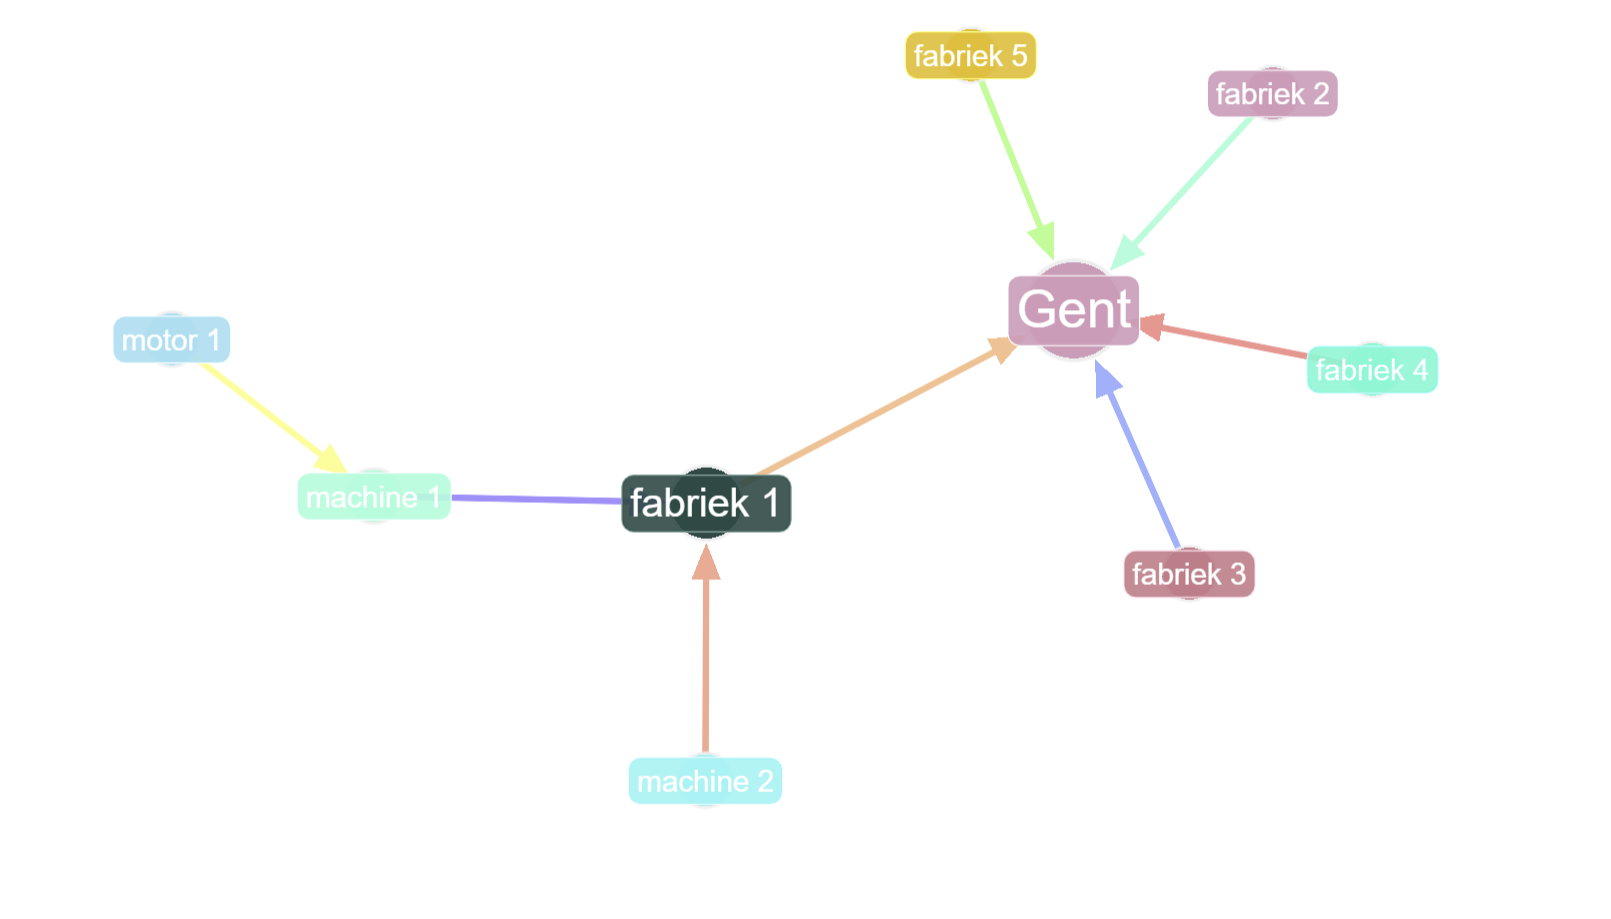
\includegraphics[width=1.0\linewidth]{./img/grapmodel_example.png}
  \captionof{figure}{Een voorbeeld van een grafiekmodel dat gebruikt wordt in deze bachelorproef.}
\end{center}

\section{Conclusies}
In deze bachelorproef is onderzocht hoe een combinatie van een grafiekmodel en een Large Language Model (LLM) kan worden ingezet om gegevens binnen het staalverwerkingsproces van ArcelorMittal Gent efficiënt op te vragen.
Het doel was een proof of concept te ontwikkelen die niet alleen de traceerbaarheid van productieprocessen verbetert, maar ook de operationele efficiëntie verhoogt door middel van een chatbot die procesvragen kan beantwoorden.
Door de SAP-boomstructuur om te zetten naar JSON-LD-formaat volgens GS1-standaarden en deze te structureren in een grafiekdatabase (Cosmos DB), werd een stevige basis gelegd voor het traceren van productieprocessen.
Vervolgens werd een chatbot ontwikkeld die gebruikmaakt van Gremlin-queries en Retrieval Augmented Generation (RAG) om procesvragen te vertalen naar begrijpelijke antwoorden.
Met modellen zoals Code Llama voor querygeneratie en Phi-4 voor natuurlijke taalverwerking is een performante oplossing opgezet die uitbreidbaar is en bruikbaar voor andere use-cases binnen de industrie.


\section{Toekomstig onderzoek}

Om de chatbot verder uit te breiden en te verbeteren, kunnen verschillende zaken worden aangepakt.
Allereerst kan gekeken worden naar het finetunen van het CodeLlama-model met LoRA, om de kwaliteit van de gegenereerde Gremlin-queries te verbeteren.
Daarnaast kunnen er nog meer prestatieoptimalisaties worden doorgevoerd om de snelheid van de chatbot te verhogen.

Ook kunnen rechten worden toegevoegd, zodat bepaalde gebruikersgroepen alleen specifieke vragen kunnen stellen of antwoorden kunnen ontvangen.
Daarnaast kunnen deze rechten worden gebruikt om DELETE-, ADD- en UPDATE-acties toe te voegen, waardoor de chatbot multifunctioneel wordt.

\end{multicols}
\end{document}